\chapter{Design}





The development of a Natural Language Interface to Database (NLIDB) System comprises of the following two systems\cite{eight}:

\begin{itemize}

\item \textbf{Linguistic component}\\
The objective of this component is to translate natural language input SQL query and hence generate the data asked by querying the database.

\item \textbf{Database component}\\
This component performs the Database Management functions. Where a lexicon is used to map the words from the natural query to database relation names, attribute names and some constraint relationship (eg. Foreign Key - Primary Key relationship). Generated parse tree for natural language query is then mapped to database objects using semantic interpreter with the help of lexicon. And a natural language generator is used to parse the resultant parse tree to generate a natural language response. Questions entered in natural language translated into a statement in a formal query language. Once the statement unambiguously formed with the help of user interaction. Then query is given to database management system and after processing desired data is generated.

\begin{figure}[htp]
\center
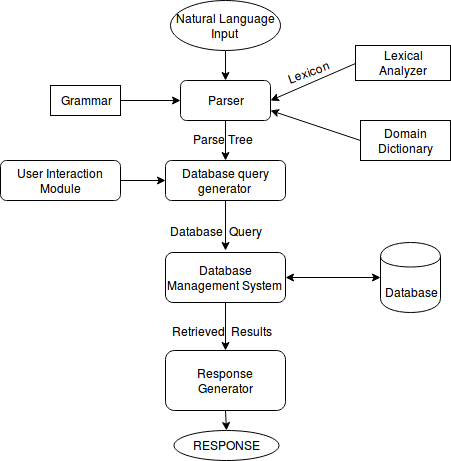
\includegraphics[width=0.5\columnwidth]{newHLL}
\caption{High level design.}
\label{fig:High level design}
\end{figure}

\item The natural language input is first processed syntactically by the parser. A parse tree is generated by parser using syntax rules from grammar. User interaction is used to remove any ambiguity in query input.

\item Then using semantic interpreter parse tree is transformed in an intermediate logic query. The semantics rule computes the logic expression of left nodes of the syntax rule, as a function of the logic expressions of the right-hand side of the syntax rule. The logic expressions corresponding to words are declared in the lexicon.\cite{two}

\item The semantic interpreter also consults a world model, that describes the structure of the surrounding world. Typically, the world model contains a hierarchy of classes of world objects, and constraints on the types of arguments each logic predicate may have.\cite{two}

\item The logic query generated by the parsing and semantic interpretation module, expresses the meaning of the user’s question in terms of logical, high-level concepts. Database query generator transforms logical to SQL query using mapping to database information.

\item Generated SQL query is given as input to underlying DBMS in order to retrieve requested data from database. DBMS queries the database and generated response is passed to the response generator. Responsibility of the response generator is to provide fetched result from database to user.

\item \textbf{Generation of the Domain Dictionary} \\
Dictionaries used by existing NLIDBs are created manually or semi-automatically. We can automate the generation of the domain dictionary from a synonym dictionary and the database metadata with the help of some linguistic processing.

\begin{figure}[ht]
\center
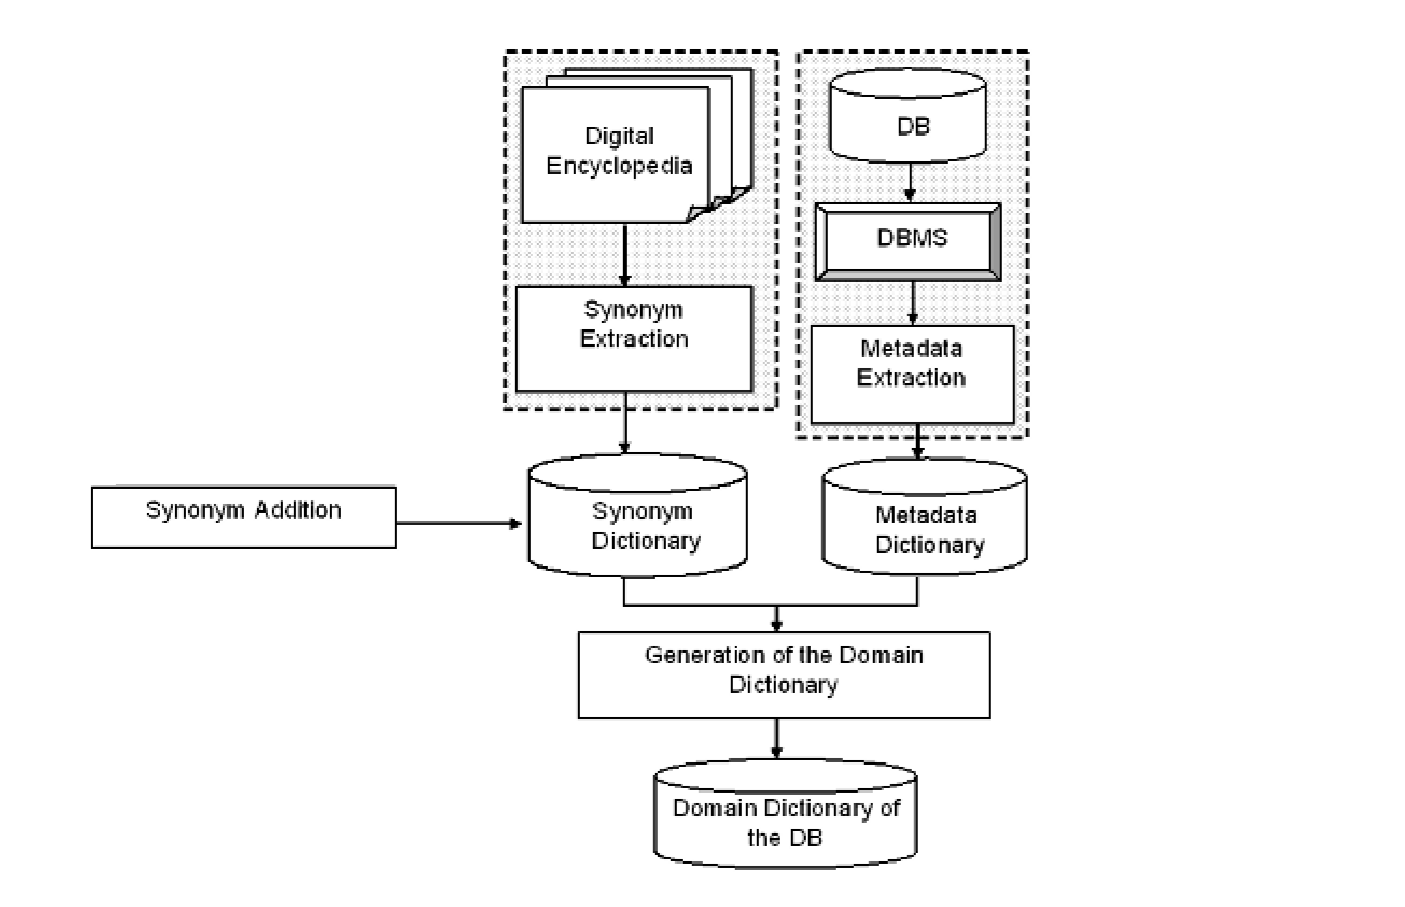
\includegraphics[width=1\columnwidth]{Dictionary}
\caption{Generation of domain dictionary}
\label{fig:Generation of domain dictionary}
\cite{five}
\end{figure}

\item \textit{Synonym dictionary}\\
A general synonym dictionary can be extracted from a digital encyclopedia. Encyclopedia contains synonyms and antonyms of thousands of the words. This dictionary can be used for most domains to better interpret query. WordNet\cite{aaa} is an example for such encyclopedia which can also be used for this purpose.

\item \textit{Metadata dictionary}\\
Queries to database are restricted to database domain. So a dictionary generated from database can be used for better mapping of natural language query to database relations and attributes.  The metadata dictionary store database information such as number of tables, number of columns, and its location. Additionally, for each table it stores the name of each column along with its data type and description, which contains primary key and foreign key information used to translate a complex query using join operations.

\item \textit{Domain dictionary}\\
For automatic generation of the domain dictionary, the description of each column from the metadata dictionary is processed to obtain the lemma and the part of speech (POS) of each word in the description.
\end{itemize}


